\PassOptionsToPackage{table}{xcolor}
\documentclass{beamer}\usepackage[]{graphicx}\usepackage[]{color}
%% maxwidth is the original width if it is less than linewidth
%% otherwise use linewidth (to make sure the graphics do not exceed the margin)
\makeatletter
\def\maxwidth{ %
  \ifdim\Gin@nat@width>\linewidth
    \linewidth
  \else
    \Gin@nat@width
  \fi
}
\makeatother

\definecolor{fgcolor}{rgb}{0.345, 0.345, 0.345}
\newcommand{\hlnum}[1]{\textcolor[rgb]{0.686,0.059,0.569}{#1}}%
\newcommand{\hlstr}[1]{\textcolor[rgb]{0.192,0.494,0.8}{#1}}%
\newcommand{\hlcom}[1]{\textcolor[rgb]{0.678,0.584,0.686}{\textit{#1}}}%
\newcommand{\hlopt}[1]{\textcolor[rgb]{0,0,0}{#1}}%
\newcommand{\hlstd}[1]{\textcolor[rgb]{0.345,0.345,0.345}{#1}}%
\newcommand{\hlkwa}[1]{\textcolor[rgb]{0.161,0.373,0.58}{\textbf{#1}}}%
\newcommand{\hlkwb}[1]{\textcolor[rgb]{0.69,0.353,0.396}{#1}}%
\newcommand{\hlkwc}[1]{\textcolor[rgb]{0.333,0.667,0.333}{#1}}%
\newcommand{\hlkwd}[1]{\textcolor[rgb]{0.737,0.353,0.396}{\textbf{#1}}}%

\usepackage{framed}
\makeatletter
\newenvironment{kframe}{%
 \def\at@end@of@kframe{}%
 \ifinner\ifhmode%
  \def\at@end@of@kframe{\end{minipage}}%
  \begin{minipage}{\columnwidth}%
 \fi\fi%
 \def\FrameCommand##1{\hskip\@totalleftmargin \hskip-\fboxsep
 \colorbox{shadecolor}{##1}\hskip-\fboxsep
     % There is no \\@totalrightmargin, so:
     \hskip-\linewidth \hskip-\@totalleftmargin \hskip\columnwidth}%
 \MakeFramed {\advance\hsize-\width
   \@totalleftmargin\z@ \linewidth\hsize
   \@setminipage}}%
 {\par\unskip\endMakeFramed%
 \at@end@of@kframe}
\makeatother

\definecolor{shadecolor}{rgb}{.97, .97, .97}
\definecolor{messagecolor}{rgb}{0, 0, 0}
\definecolor{warningcolor}{rgb}{1, 0, 1}
\definecolor{errorcolor}{rgb}{1, 0, 0}
\newenvironment{knitrout}{}{} % an empty environment to be redefined in TeX

\usepackage{alltt}

\mode<presentation>
{
  \usetheme{Warsaw}
  
}

\beamertemplatenavigationsymbolsempty 

\usepackage[]{inputenc}
\usepackage[english]{babel}
\usepackage{amsthm}
\usepackage{graphicx}
\usepackage{epstopdf}
\usepackage{grffile}
\usepackage{hyperref}
\usepackage{beamerthemesplit}
\definecolor{links}{HTML}{2A1B81}
\hypersetup{colorlinks,linkcolor=,urlcolor=links}
%\setsansfont[Ligatures={Common,TeX}]{TeX Gyre Heros}

{\renewcommand{\arraystretch}{1.1}

\AtBeginSection[]
{
  \begin{frame}
    \frametitle{Outline}
    \tableofcontents[currentsection]
  \end{frame}
}

\newcommand*\oldmacro{}%
\let\oldmacro\insertshorttitle%
\renewcommand*\insertshorttitle{%
   \oldmacro\hfill%
   \insertframenumber\,/\,\inserttotalframenumber}

\setbeamertemplate{headline}{}
\setbeamertemplate{itemize items}[circle]
\title{Statistical Analysis of \texttt{Illumina} merged pair reads}

\author [Andrew Bzikadze]{Andrew Bzikadze\\ \texttt{\small{\href{mailto:seryrzu@gmail.com}{seryrzu@gmail.com}}}}
%\institute{Saint Petersburg State University, Russia \\
%           Faculty of Mathematics and Mechanics \\
%           Department of Statistical Modelling}
\date {
September 13, 2015
}

\usepackage[absolute,overlay]{textpos}
\setlength{\TPHorizModule}{1cm} % Horizontale Einheit
\setlength{\TPVertModule}{1cm} % Vertikale Einheit
\addtobeamertemplate{title page}{
}{}
\IfFileExists{upquote.sty}{\usepackage{upquote}}{}

\begin{document}
\begin{frame}
  \titlepage
\end{frame}

\section{Introduction}
\begin{frame}{Introduction}
  \textbf{Research direction:} analysis of input merged pair reads using statistical and simulation methods.
  
  \pause 
  \textbf{Questions:}
  \begin{itemize}
    \item What is the distribution law of nucleotide subsequences of merged pair reads?
    \item Is there any correlation between biological events (for instance, between \textit{cleavage} / \textit{palindromes} and specific gene segments)?
    \item What model describes biological events the best (for example, \textit{insertions} at the \texttt{VD}-, \texttt{DJ}- junction)? 
  \end{itemize}
\end{frame}

\begin{frame}{Motivation}
  \textbf{Motivation:} knowledge of the distribution of nucleotide sequences potentially helps with
  \begin{itemize}
    \item Simulation of pair reads: improvements of \texttt{IgSimulator}.
    \item Dealing with Clonal Trees. ???
    \item Comparison of different antibody repertoires.
    \item String metrics for measuring the difference between two sequences: improvements of \texttt{IgRepertoireConstructor}.
  \end{itemize}
\end{frame}

\begin{frame}{Background}
  An article about the distribution law of \texttt{CDR3} generating recombinations for \texttt{T}-cells:
  
  \href{http://www.pnas.org/content/109/40/16161.full}{%Statistical inference of the generation probability of \texttt{T}-cell receptors from sequence repertoires (
  Anand Murugana, Thierry Morab, Aleksandra M. Walczakc and Curtis G. Callan --- 2012}:
  \begin{itemize}
    \item Analysis is focused on nonproductive \texttt{CDR3}.
    \item Suggested model sets joint distribution over the set of discrete variables: \textit{identities} of \texttt{V-, D-, J-} gens, number of \textit{deletions} from the end of a segment, \textit{palindromic} nucleotides and \textit{insertions} at the end of a gen.
    \pause
  \item {\color{blue} 2865(!) parametrs to estimate.}
  \end{itemize}
\end{frame}

\begin{frame}{Background}
  \textbf{Questions about the paper:}
  \begin{itemize}
    \item Is the suggested model really adequate (including the problem of potential overfitting)?
    \item Are the results statistically significant?
    \item Are similar results true for \texttt{B}-cells?
  \end{itemize}
 
  \pause
  \bigskip
  {\color{blue} Difficult to answer, should start with something simpler.}
\end{frame}

\begin{frame}{Two types of events}
  It is reasonable to classify events (palindromes, cleavage, etc.) into ``{\color{blue} biological}'' and ``{\color{blue} accidental}''.
  
  \textbf{Example:} if we detect a palindrome at the end of a segment, while clavage has also happened, then we defenitely detect an \textit{accidental} (noise) palindrome.
\bigskip

  The goals 
  \begin{itemize}
    \item correlations between palindromes and specific gene segments;
    \item distribution law of nucleotide subsequences
  \end{itemize}
  include the task of classification the events into two types and hence require some additional knowledge about the structure of the repertoire.
 
  \bigskip
  Considering that and the questions about the article let's firstly concentrate on a simplier problem of seeking \textbf{correlation between cleavage and specific gene segments.} 
\end{frame}

\section{Cleavage and specific gene segments}
\begin{frame}{Cleavage and specific gene segments}
  \textbf{Problem:} In the datasets not only \texttt{V(D)J}-recombinations effects are reflected, but also the result of ????.
 
  \pause
  %\textbf{Idea:} Let's take only gens, that align to the germline with  level at least $C$, where $0 \leqslant C \leqslant 1$.
  \bigskip 
  \textbf{Scheme:}
  \begin{itemize}
    \item Consider a merged pair dataset.
    \pause
    \item Use \texttt{IgRepertoireConstructor} for this dataset and consider {\color{blue} highly abundant antibody clusters} of the constructed repertoire.
    \pause
    \item Apply \texttt{IgBlast} to reads from highly abundant clusters.
    \pause
    \item {\color{blue} Downsampling}: consider only such reads, that have alignment score of their segments not less than a {\color{blue} threshold} according to \texttt{IgBlast}.
  \end{itemize}

  \bigskip
  {\color{blue} Scheme is invariant of biological event we are interested in.}
\end{frame}

\begin{frame}{Cleavage and specific gene segments: \texttt{V}-gens}
 \begin{figure}[h]
  \begin{minipage}[h]{0.49\linewidth}
    \center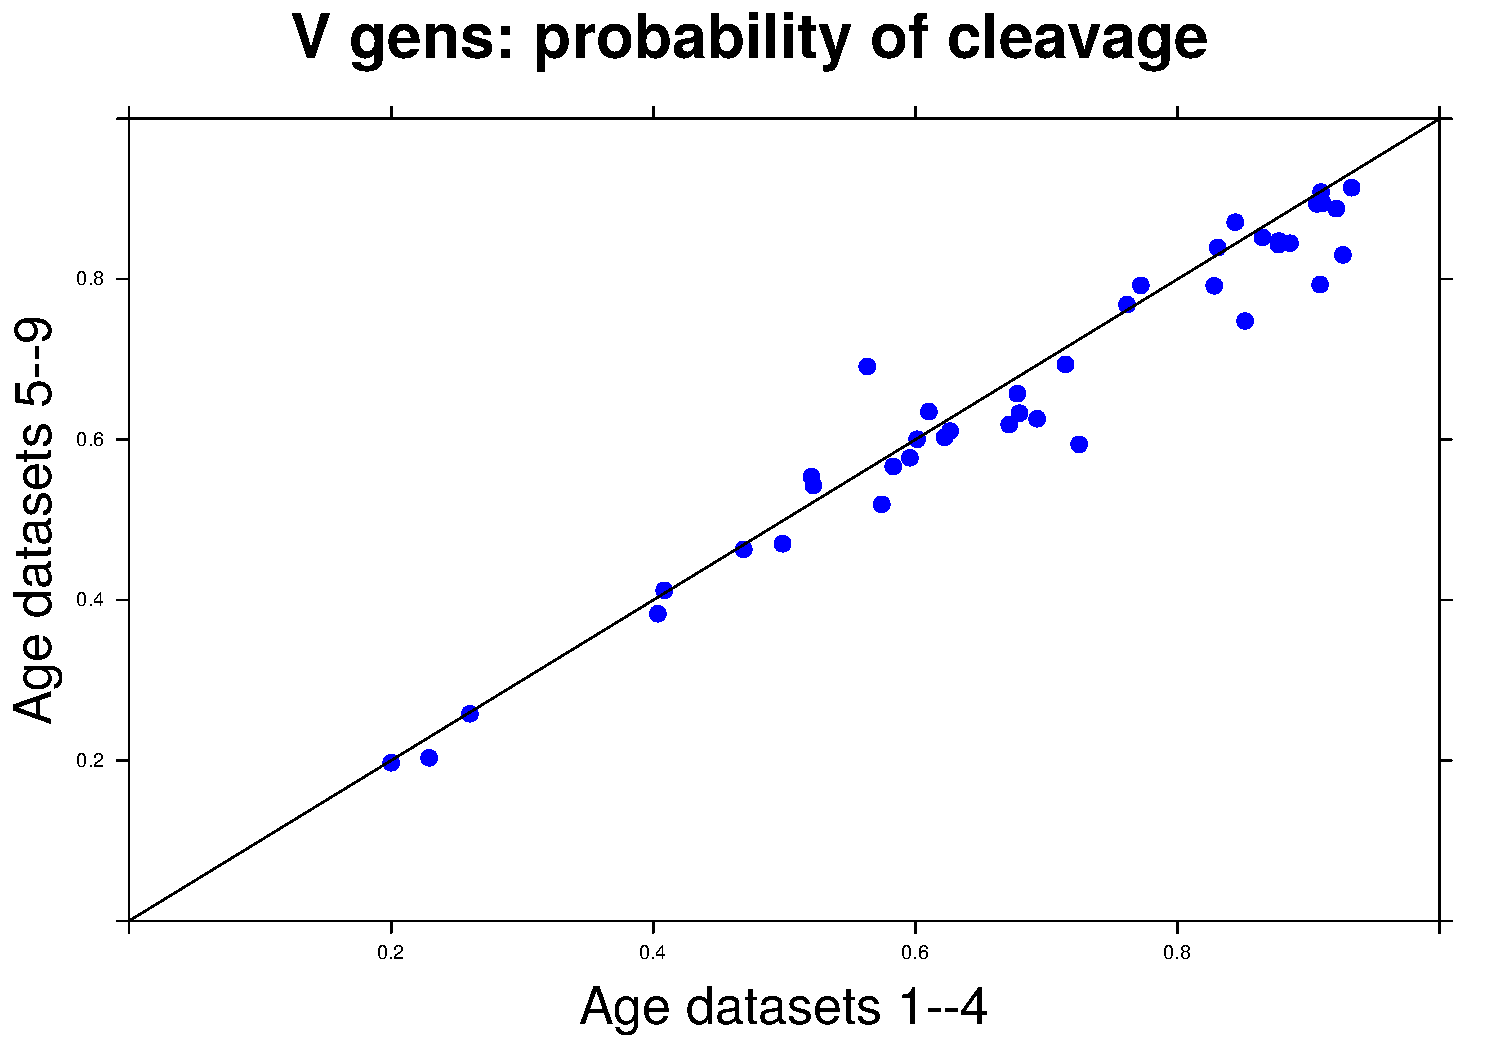
\includegraphics[width=150pt]{Vgen_cleavage_age.pdf}
    \caption{\footnotesize{\texttt{Age} datasets. The point --- is the gen. Pearson correlation is $0.98$.}} 
  \end{minipage}
  \hfill
  \begin{minipage}[h]{0.49\linewidth}
   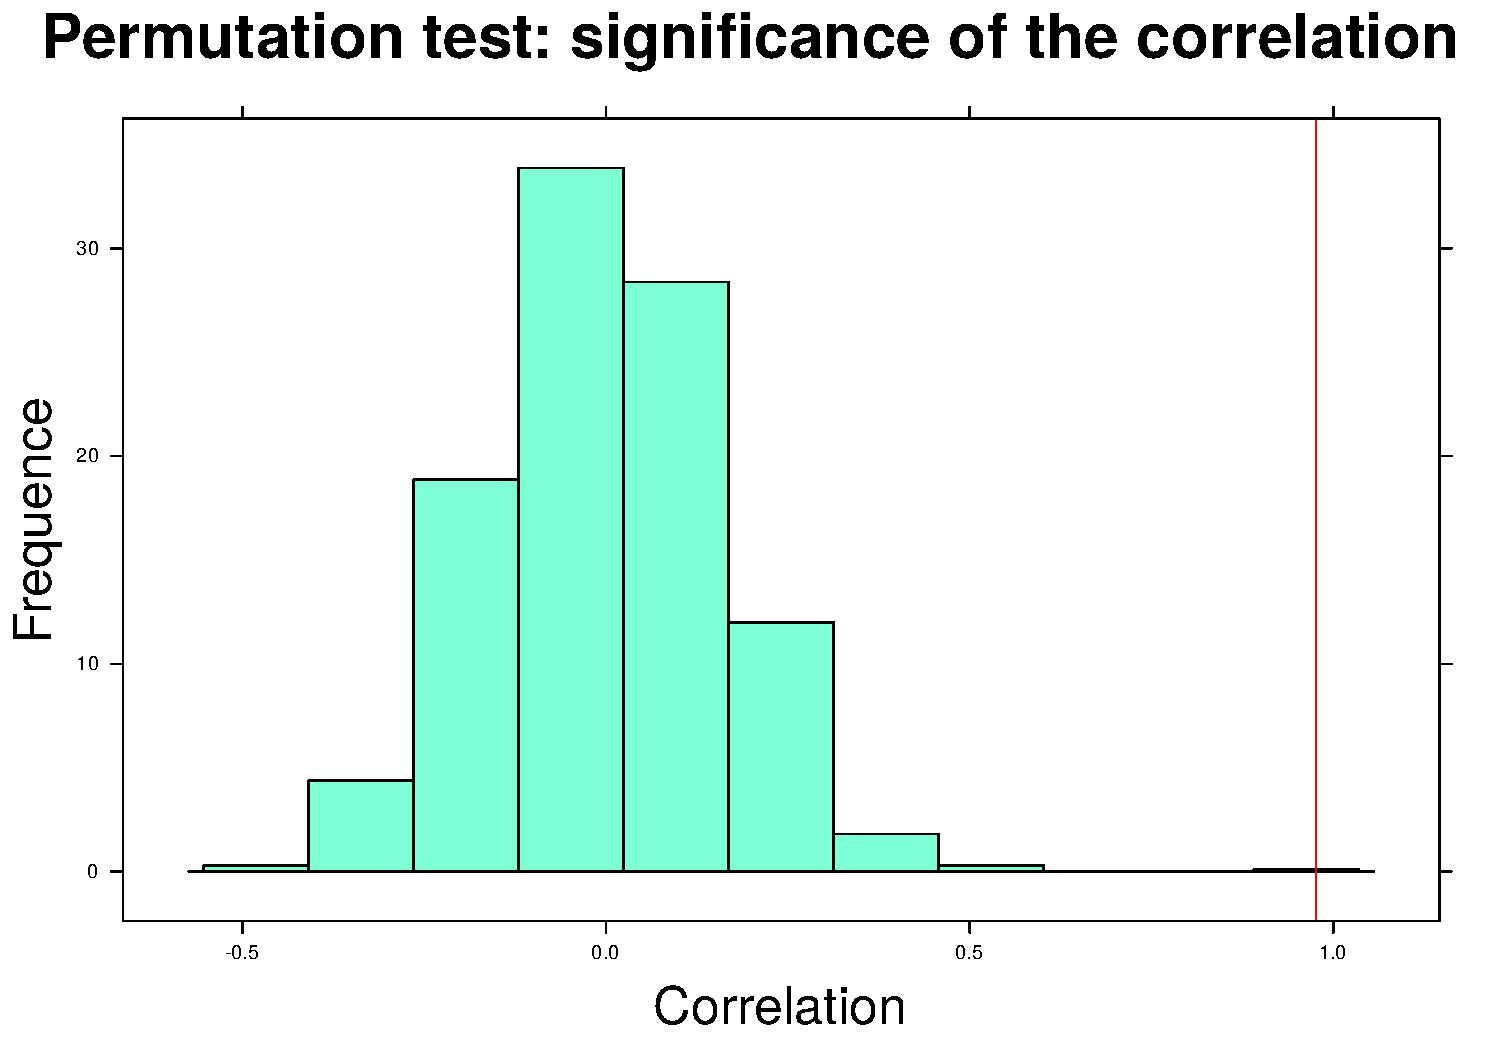
\includegraphics[width=150pt]{Vgen_cleavage_age_correlation.pdf}
    \caption{\footnotesize{Histogram of statistics of permutation test that shows the significance of Pearson correlation.}} 
  \end{minipage}
 \end{figure}
 \pause
 {\color{blue} Hence reads in the dataset are dependent standart pooled $Z$-test for equal propotions is not applicable.}
 \pause
 
 \textbf{Remark:} No obvious way to clusterize $V$-gens effectively.
\end{frame}

\begin{frame}{Further goals to clusterize gens}
  As long as the probabilities of cleavage for gens don't introduce an obvious way to clusterize $V$-gens (and hence to reduce the number of parameters in the model for distribution)
  the next steps will be correlations between the gen and
  \begin{itemize}
    \item \textit{palindromes} length;
    \item \texttt{GC}-content;
    \item different type of gens (\texttt{V} vs \texttt{J} \textit{etc}.)
    \item ???
  \end{itemize}
\end{frame}

\section{Two types of palindromes}
\begin{frame}{Two types of palindromes}
  It is known that if cleavage took place, then no palindrome can happen. This is only partially true. 
  ``{\color{blue} Accidental}'' palindrome can still happen, but it won't have ``{\color{blue} biological}'' nature.
  
  \bigskip
  \begin{itemize}
    \item The simplest model is that nucletides are distributed \textbf{uniformly}.
    \item In that model the length of ``accidental'' palindrome has $\mathrm{Geom}(3/4)$ distribution.
  \end{itemize}
  
  %\bigskip
  %\pause
  %{\color{blue} If ``biological'' palindrome has different distribution, maybe it will be possible to construct one.}
\end{frame}

\begin{frame}{Two types of palindromes}
 Emperical (\texttt{Age}-datasets) and theoretical distribution in $\log$ scale:
 \begin{figure}[h]
  \begin{minipage}[h]{0.49\linewidth}
    \center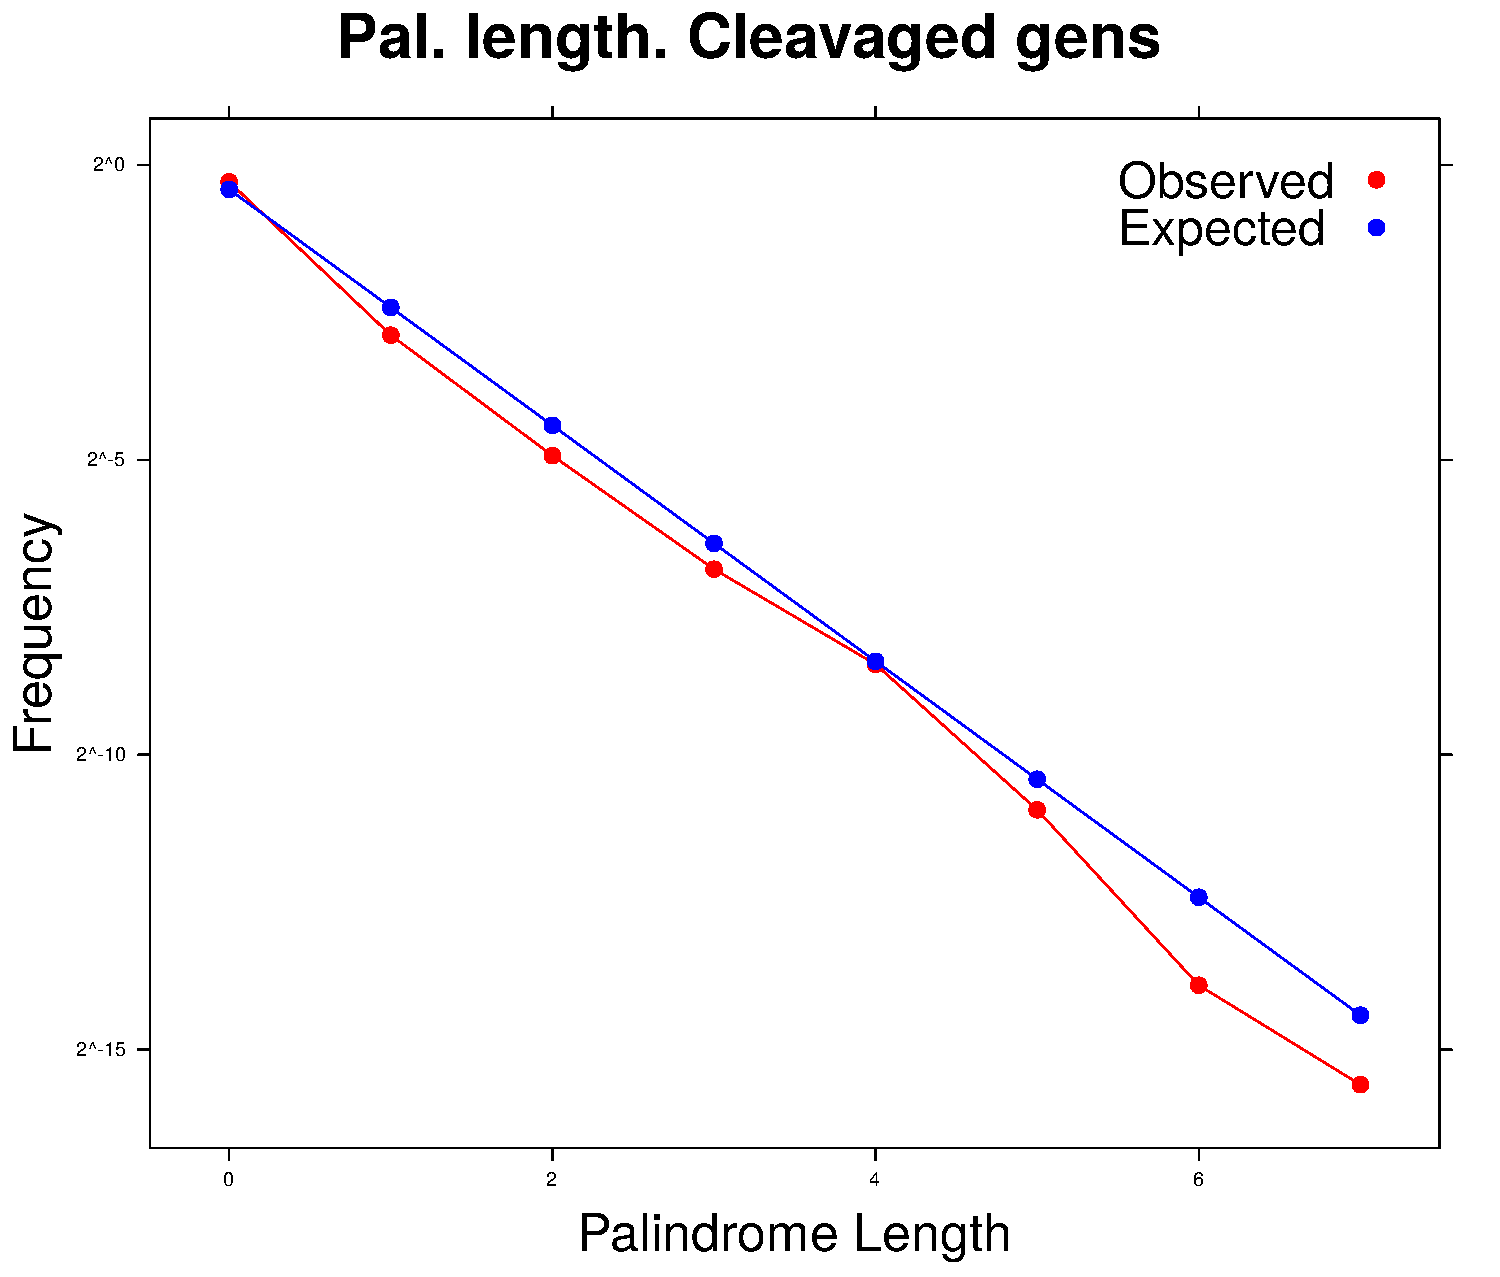
\includegraphics[width=150pt]{distr_pal_len_cl.pdf}
    \caption{\footnotesize{The $\mathrm{mean}$  of length is $0.33$.}}
  \end{minipage}
  \hfill
  \begin{minipage}[h]{0.49\linewidth}
   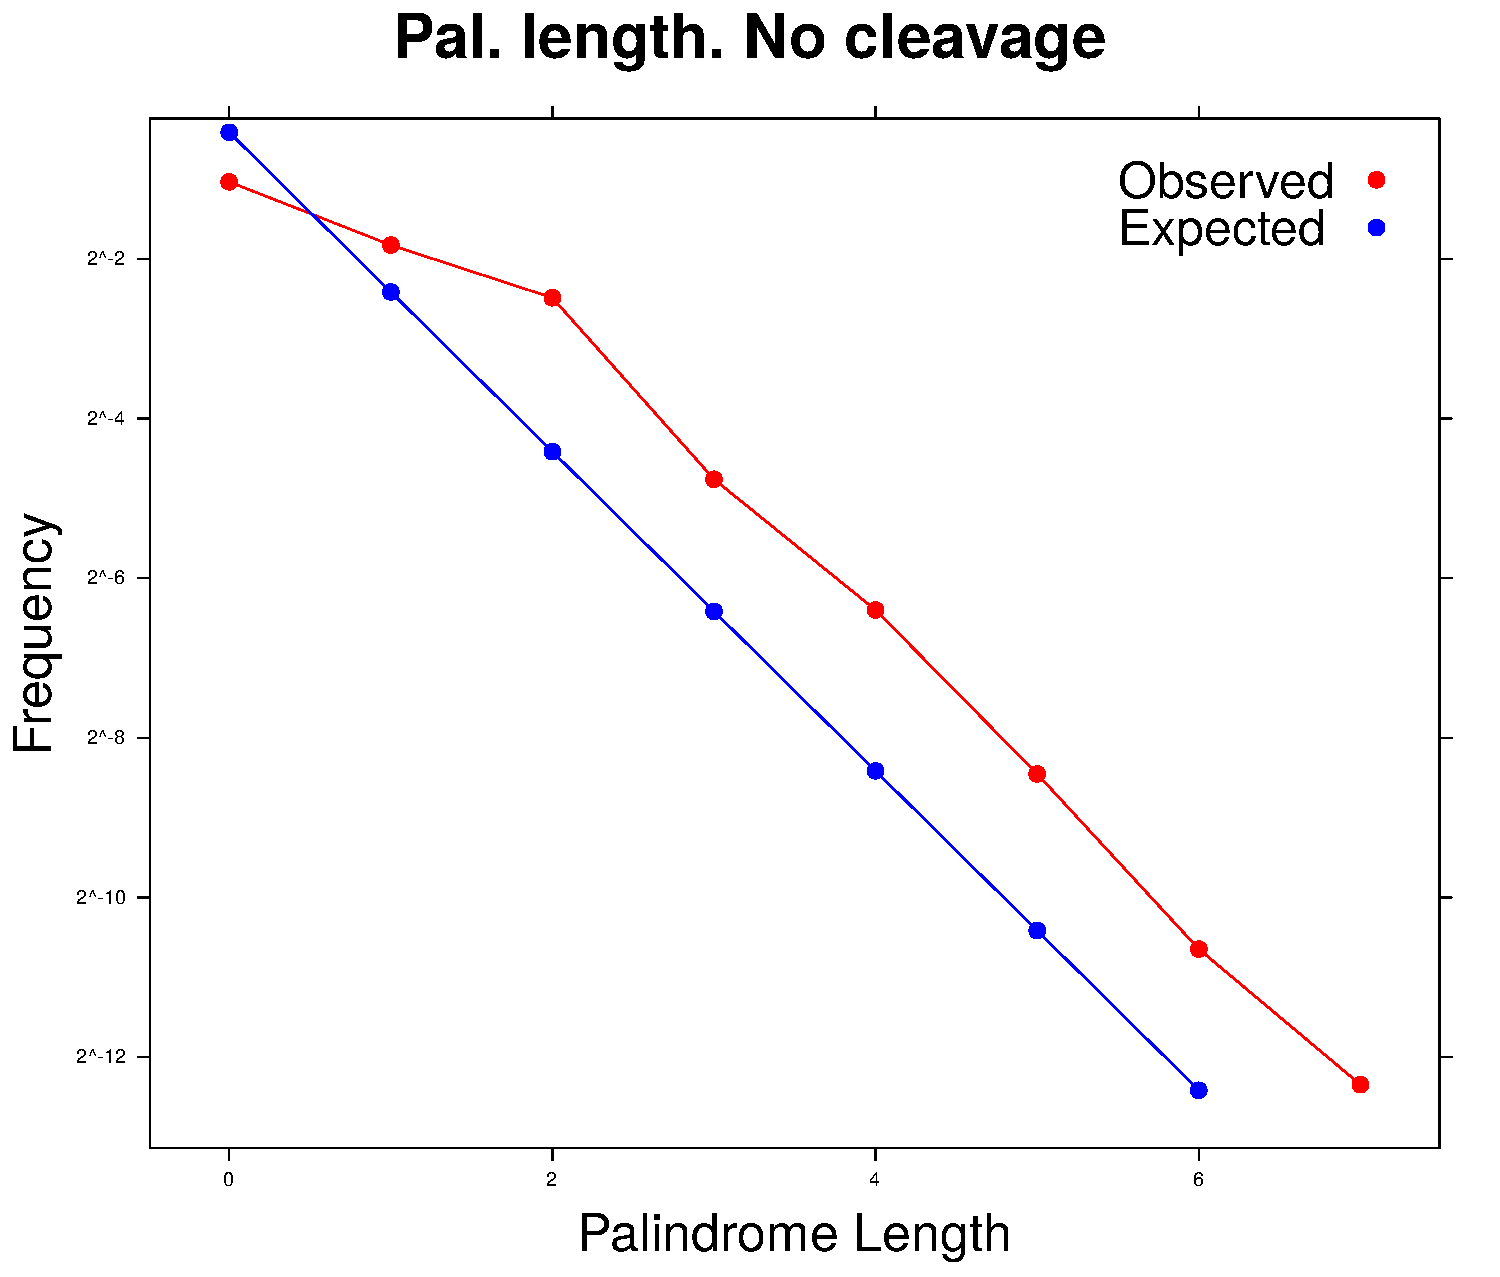
\includegraphics[width=150pt]{distr_pal_len_nocl.pdf}
   \caption{\footnotesize{The $\mathrm{mean}$ of length is $0.82$.}} 
  \end{minipage}
 \end{figure}
 
 \pause
 {\color{blue} Hence reads in the dataset are dependent goodness-of-fit $\chi^2$-test is not applicable. }
\end{frame}


\begin{frame}{What else about the palindromes}
  \begin{itemize}
    \item To find out the distribution of ``biological'' palindrome.
    \item To construct more adequate model for nucleotide distribution.
    \item ???
  \end{itemize}
\end{frame}

\section{}
\begin{frame}{Next steps}
  To sum up let's revisit main important questions:
  \begin{itemize}
    \item What is the distribution of the nucleotides?
    \item What events are correlated strongly / weakly with each other?
    \item How to distinguish ``biological'' and ``accidental'' events?
  \end{itemize}
  \bigskip
  Also checking whether the model advised in the \href{http://www.pnas.org/content/109/40/16161.full}{%Statistical inference of the generation probability of \texttt{T}-cell receptors from sequence repertoires (
  article} is adequate for \texttt{B}-cells (and trying to reduce the number of the parametrs) seems to be reasonable.


  \bigskip
  Further analysis will be concentrated on this problems.
\end{frame}


\end{document}
